\documentclass[11pt,a4paper]{report}
\usepackage[textwidth=37em,vmargin=30mm]{geometry}
\usepackage{calc,xunicode,amsmath,amssymb,paralist,enumitem,tabu,booktabs,datetime2,xeCJK,xeCJKfntef,listings}
\usepackage{tocloft,fancyhdr,tcolorbox,xcolor,graphicx,eso-pic,xltxtra,xelatexemoji}

\newcommand{\envyear}[0]{2025}
\newcommand{\envdatestr}[0]{2025-03-12}
\newcommand{\envfinaldir}[0]{webdb/2025/20250312/final}

\usepackage[hidelinks]{hyperref}
\hypersetup{
    colorlinks=false,
    pdfpagemode=FullScreen,
    pdftitle={Web Digest - \envdatestr}
}

\setlength{\cftbeforechapskip}{10pt}
\renewcommand{\cftchapfont}{\rmfamily\bfseries\large\raggedright}
\setlength{\cftbeforesecskip}{2pt}
\renewcommand{\cftsecfont}{\sffamily\small\raggedright}

\setdefaultleftmargin{2em}{2em}{1em}{1em}{1em}{1em}

\usepackage{xeCJK,xeCJKfntef}
\xeCJKsetup{PunctStyle=plain,RubberPunctSkip=false,CJKglue=\strut\hskip 0pt plus 0.1em minus 0.05em,CJKecglue=\strut\hskip 0.22em plus 0.2em}
\XeTeXlinebreaklocale "zh"
\XeTeXlinebreakskip = 0pt


\setmainfont{Brygada 1918}
\setromanfont{Brygada 1918}
\setsansfont{IBM Plex Sans}
\setmonofont{JetBrains Mono NL}
\setCJKmainfont{Noto Serif CJK SC}
\setCJKromanfont{Noto Serif CJK SC}
\setCJKsansfont{Noto Sans CJK SC}
\setCJKmonofont{Noto Sans CJK SC}

\setlength{\parindent}{0pt}
\setlength{\parskip}{8pt}
\linespread{1.15}

\lstset{
	basicstyle=\ttfamily\footnotesize,
	numbersep=5pt,
	backgroundcolor=\color{black!5},
	showspaces=false,
	showstringspaces=false,
	showtabs=false,
	tabsize=2,
	captionpos=b,
	breaklines=true,
	breakatwhitespace=true,
	breakautoindent=true,
	linewidth=\textwidth
}






\newcommand{\coverpic}[2]{
    % argv: itemurl, authorname
    Cover photo by #2~~(\href{#1}{#1})
}
\newcommand{\makeheader}[0]{
    \begin{titlepage}
        % \newgeometry{hmargin=15mm,tmargin=21mm,bmargin=12mm}
        \begin{center}
            
            \rmfamily\scshape
            \fontspec{BaskervilleF}
            \fontspec{Old Standard}
            \fontsize{59pt}{70pt}\selectfont
            WEB\hfill DIGEST
            
            \vfill
            % \vskip 30pt
            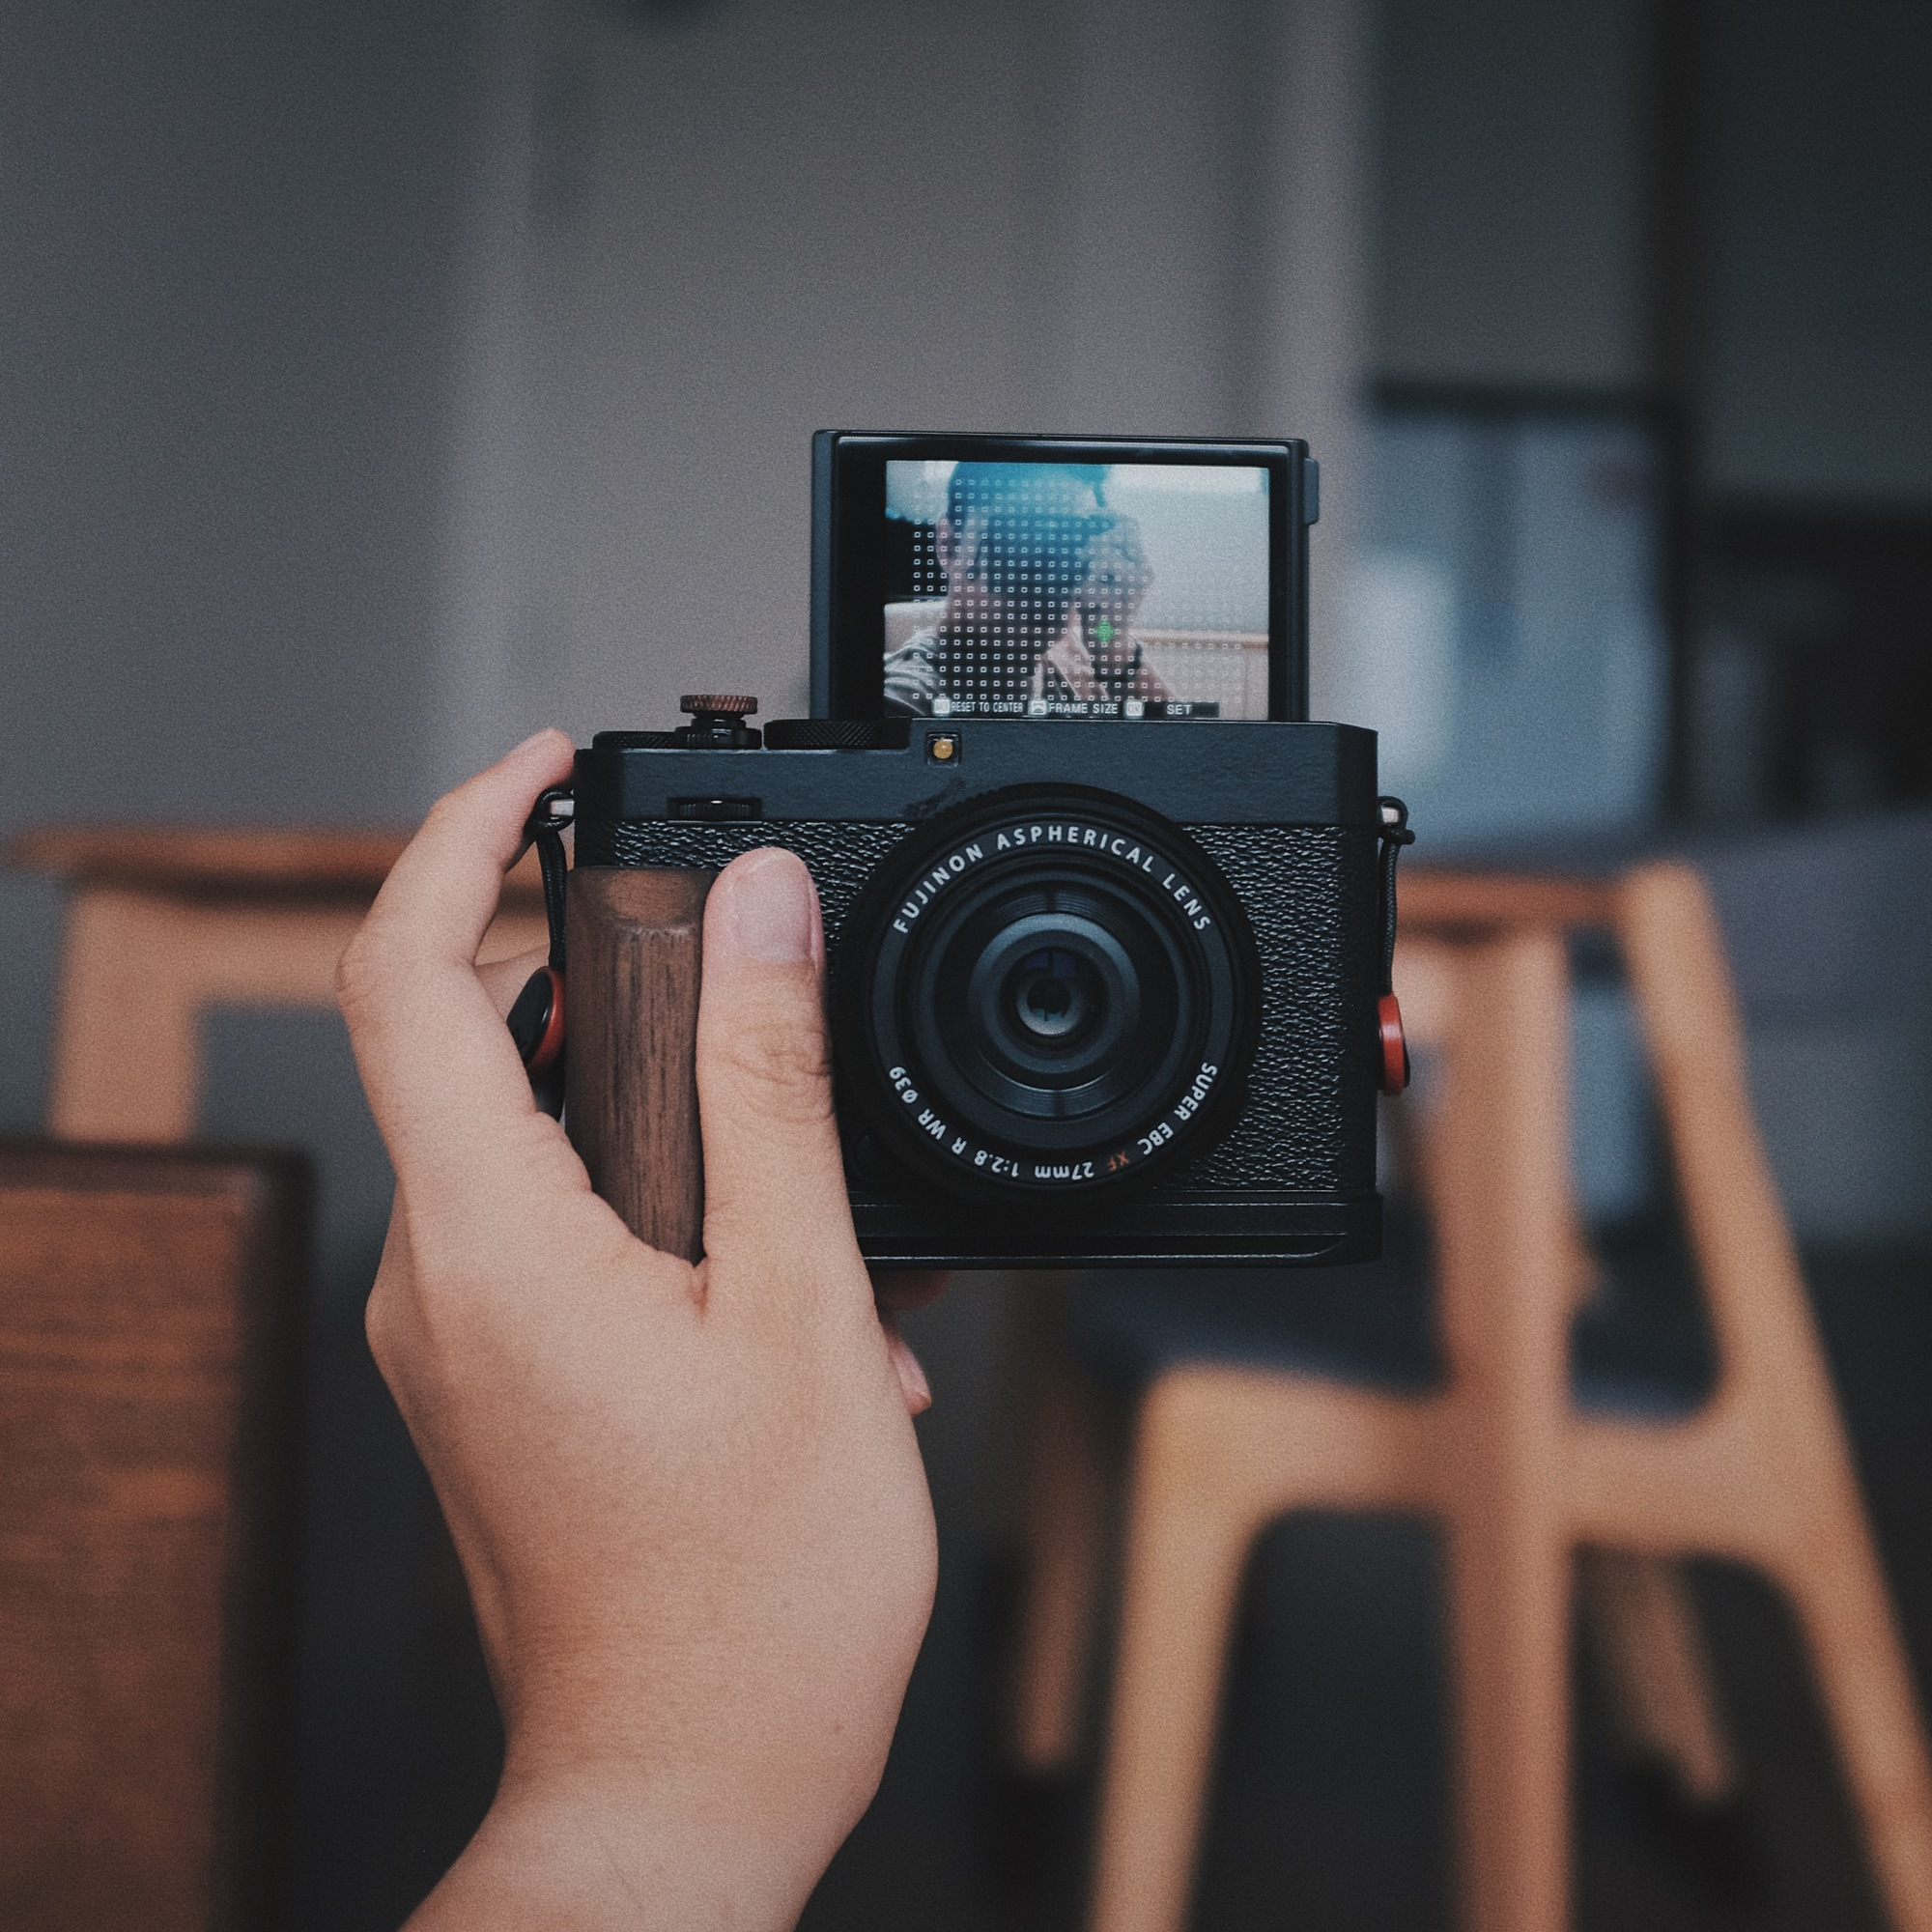
\includegraphics[width=\linewidth]{\envfinaldir/coverpic-prod.jpg}\par
            % \vskip 30pt
            \vfill

            \normalsize\rmfamily\scshape
            \copyright{} The Web Digest Project \hfill\large \envdatestr
        \end{center}
    \end{titlepage}
    % \restoregeometry
}
\newcommand{\simplehref}[1]{%
    \textcolor{blue!80!green}{\href{#1}{#1}}%
}
\renewcommand{\contentsname}{\center\Huge\sffamily\bfseries Contents\par\vskip 20pt}
\newcounter{ipartcounter}
\setcounter{ipartcounter}{0}
\newcommand{\ipart}[1]{
    % \vskip 20pt
    \clearpage
    \stepcounter{ipartcounter}
    \phantomsection
    \addcontentsline{toc}{chapter}{#1}
    % \begin{center}
    %     \Huge
    %     \sffamily\bfseries
    %     #1
    % \end{center}
    % \vskip 20pt plus 7pt
}
\newcounter{ichaptercounter}
\setcounter{ichaptercounter}{0}
\newcommand{\ichapter}[1]{
    % \vskip 20pt
    \clearpage
    \stepcounter{ichaptercounter}
    \phantomsection
    \addcontentsline{toc}{section}{\numberline{\arabic{ichaptercounter}}#1}
    \begin{center}
        \Huge
        \sffamily\bfseries
        #1
    \end{center}
    \vskip 20pt plus 7pt
}
\newcommand{\entrytitlefont}[1]{\subsection*{\raggedright\Large\sffamily\bfseries#1}}
\newcommand{\entryitemGeneric}[2]{
    % argv: title, url
    \parbox{\linewidth}{
        \entrytitlefont{#1}\par\vskip 5pt
        \footnotesize\ttfamily\mdseries
        \simplehref{#2}
    }\vskip 11pt plus 11pt minus 1pt
}
\newcommand{\entryitemGithub}[3]{
    % argv: title, url, desc
    \parbox{\linewidth}{
        \entrytitlefont{#1}\par\vskip 5pt
        \footnotesize\ttfamily\mdseries
        \simplehref{#2}\par\vskip 5pt
        \small\rmfamily\mdseries#3
    }\vskip 11pt plus 11pt minus 1pt
}
\newcommand{\entryitemAp}[3]{
    % argv: title, url, desc
    \parbox{\linewidth}{
        \entrytitlefont{#1}\par\vskip 5pt
        \footnotesize\ttfamily\mdseries
        \simplehref{#2}\par\vskip 5pt
        \small\rmfamily\mdseries#3
    }\vskip 11pt plus 11pt minus 1pt
}
\newcommand{\entryitemHackernews}[3]{
    % argv: title, hnurl, rawurl
    % \parbox{\linewidth}{
    %     \entrytitlefont{#1}\par\vskip 5pt
    %     \footnotesize\ttfamily\mdseries
    %     \simplehref{#3}\par
    %     \textcolor{black!50}{\href{#2}{#2}}
    % }\vskip 11pt plus 11pt minus 1pt
    \begin{minipage}{\linewidth}
            \entrytitlefont{#1}\par\vskip 5pt
            \footnotesize\ttfamily\mdseries
            \simplehref{#3}\par
            \textcolor{black!50}{\href{#2}{#2}}
    \end{minipage}\par\vskip 11pt plus 11pt minus 1pt
}







\begin{document}

\makeheader

\tableofcontents\clearpage




\ipart{Developers}
\ichapter{Hacker News}
\entryitemTwoLinks{Why Go?}{https://news.ycombinator.com/item?id=43334830}{https://github.com/microsoft/typescript-go/discussions/411}

\entryitemTwoLinks{New tools for building agents}{https://news.ycombinator.com/item?id=43334644}{https://openai.com/index/new-tools-for-building-agents/}

\entryitemTwoLinks{Fastplotlib: GPU-accelerated, fast, and interactive plotting library}{https://news.ycombinator.com/item?id=43334190}{https://medium.com/@caitlin9165/fastplotlib-driving-scientific-discovery-through-data-visualization-418f8bff094c}

\entryitemTwoLinks{Show HN: Krep a High-Performance String Search Utility Written in C}{https://news.ycombinator.com/item?id=43333946}{https://davidesantangelo.github.io/krep/}

\entryitemTwoLinks{Show HN: We built a Plug-in Home Battery for the 99.7\% of us without Powerwalls}{https://news.ycombinator.com/item?id=43333661}{https://pilaenergy.com}

\entryitemTwoLinks{AI-Generated Voice Evidence Poses Dangers in Court}{https://news.ycombinator.com/item?id=43333484}{https://www.lawfaremedia.org/article/ai-generated-voice-evidence-poses-dangers-in-court}

\entryitemTwoLinks{NIST selects HQC as fifth algorithm for post-quantum encryption}{https://news.ycombinator.com/item?id=43332944}{https://www.nist.gov/news-events/news/2025/03/nist-selects-hqc-fifth-algorithm-post-quantum-encryption}

\entryitemTwoLinks{A 10x Faster TypeScript}{https://news.ycombinator.com/item?id=43332830}{https://devblogs.microsoft.com/typescript/typescript-native-port/}

\entryitemTwoLinks{The US island that speaks Elizabethan English}{https://news.ycombinator.com/item?id=43332752}{https://www.bbc.com/travel/article/20190623-the-us-island-that-speaks-elizabethan-english}

\entryitemTwoLinks{Happy 20th Birthday, Y Combinator}{https://news.ycombinator.com/item?id=43332658}{https://twitter.com/garrytan/status/1899092996702048709}

\entryitemTwoLinks{Mapping the University of Chicago's 135-year expansion into Hyde Park and beyond}{https://news.ycombinator.com/item?id=43332424}{https://chicagomaroon.github.io/data-visualizations/2025/uchicago-property/}

\entryitemTwoLinks{Show HN: Factorio Learning Environment – Agents Build Factories}{https://news.ycombinator.com/item?id=43331582}{https://jackhopkins.github.io/factorio-learning-environment/}

\entryitemTwoLinks{America Is Missing The New Labor Economy – Robotics Part 1}{https://news.ycombinator.com/item?id=43331358}{https://semianalysis.com/2025/03/11/america-is-missing-the-new-labor-economy-robotics-part-1/}

\entryitemTwoLinks{What makes code hard to read: Visual patterns of complexity (2023)}{https://news.ycombinator.com/item?id=43330900}{https://seeinglogic.com/posts/visual-readability-patterns/}

\entryitemTwoLinks{ESP32 Undocumented Bluetooth Commands: Clearing the Air}{https://news.ycombinator.com/item?id=43330331}{https://developer.espressif.com/blog/2025/03/esp32-bluetooth-clearing-the-air/}

\entryitemTwoLinks{New Zealand's \$16B health dept managed finances with single Excel spreadsheet}{https://news.ycombinator.com/item?id=43330206}{https://www.theregister.com/2025/03/10/nz\_health\_excel\_spreadsheet/}

\entryitemTwoLinks{Local Deep Research – ArXiv, wiki and other searches included}{https://news.ycombinator.com/item?id=43330164}{https://github.com/LearningCircuit/local-deep-research}

\entryitemTwoLinks{Extreme poverty in India has dropped to negligible levels}{https://news.ycombinator.com/item?id=43329373}{https://www.economist.com/finance-and-economics/2025/02/27/india-has-undermined-a-popular-myth-about-development}

\entryitemTwoLinks{Show HN: Seven39, a social media app that is only open for 3 hours every evening}{https://news.ycombinator.com/item?id=43328095}{https://www.seven39.com}

\entryitemTwoLinks{Shef}{https://news.ycombinator.com/item?id=43327758}{https://github.com/eduardoagarcia/shef}\ichapter{Phoronix}
\entryitemGeneric{\hskip 0pt{}Intel Overclocking Watchdog Driver Posted For The Linux Kernel}{https://www.phoronix.com/news/Intel-Overclocking-Watchdog}

\entryitemGeneric{\hskip 0pt{}Nouveau On NVIDIA Turing GPUs \& Newer Will Now Prefer NVK+Zink For OpenGL}{https://www.phoronix.com/news/Nouveau-Turing-Zink-NVK-OpenGL}

\entryitemGeneric{\hskip 0pt{}CrossOver 25.0 Announced - Built Atop Wine 10.0 For Linux \& macOS}{https://www.phoronix.com/news/CrossOver-25.0-Released}

\entryitemGeneric{\hskip 0pt{}AMD Ryzen 9 9950X3D Delivers Excellent Performance For Linux Developers, Creators \& Technical Computing}{https://www.phoronix.com/review/amd-ryzen-9-9950x3d-linux}

\entryitemGeneric{\hskip 0pt{}GNOME Dash To Panel Extension Development Being "Passed On"}{https://www.phoronix.com/news/GNOME-Dash-To-Panel-Pause}

\entryitemGeneric{\hskip 0pt{}COBOL Language Frontend Merged For GCC 15 Compiler}{https://www.phoronix.com/news/GCC-15-Merges-COBOL}

\entryitemGeneric{\hskip 0pt{}Linux Kernel Patches Posted For The ESWIN EIC7700 SoC + SiFive HiFive Premier P550}{https://www.phoronix.com/news/Linux-Patches-EIC7700-HiFive}

\entryitemGeneric{\hskip 0pt{}Servo Makes Improvements To Its Demo Browser \& Embedding API}{https://www.phoronix.com/news/Servo-February-2025}

\entryitemGeneric{\hskip 0pt{}AMD Announces The EPYC Embedded 9005 Series}{https://www.phoronix.com/news/AMD-EPYC-Embedded-9005-Turin}\ichapter{Dribbble}
\entryitemGeneric{\hskip 0pt{}Triceratops}{https://dribbble.com/shots/25749787-Triceratops}

\entryitemGeneric{\hskip 0pt{}Crystal // Website}{https://dribbble.com/shots/25742820-Crystal-Website}

\entryitemGeneric{\hskip 0pt{}Emergency App Concept Design}{https://dribbble.com/shots/25711688-Emergency-App-Concept-Design}

\entryitemGeneric{\hskip 0pt{}ABN-AMRO - Logo Redesign}{https://dribbble.com/shots/25743181-ABN-AMRO-Logo-Redesign}

\entryitemGeneric{\hskip 0pt{}OneC1 - Logo Design}{https://dribbble.com/shots/25732400-OneC1-Logo-Design}

\entryitemGeneric{\hskip 0pt{}Heyo® Monograms}{https://dribbble.com/shots/25732379-Heyo-Monograms}

\entryitemGeneric{\hskip 0pt{}Best Friends}{https://dribbble.com/shots/25730832-Best-Friends}

\entryitemGeneric{\hskip 0pt{}Ecommerce illustration}{https://dribbble.com/shots/25734258-Ecommerce-illustration}

\entryitemGeneric{\hskip 0pt{}Free Fly Apparel}{https://dribbble.com/shots/25727838-Free-Fly-Apparel}

\entryitemGeneric{\hskip 0pt{}Columbus Rapids® C-Wave}{https://dribbble.com/shots/25727535-Columbus-Rapids-C-Wave}

\entryitemGeneric{\hskip 0pt{}Bloodhound Detective}{https://dribbble.com/shots/25726401-Bloodhound-Detective}

\entryitemGeneric{\hskip 0pt{}QLOUD - Logo Redesign}{https://dribbble.com/shots/25726630-QLOUD-Logo-Redesign}

\entryitemGeneric{\hskip 0pt{}Faithful web design}{https://dribbble.com/shots/25723024-Faithful-web-design}

\entryitemGeneric{\hskip 0pt{}Dj Dule logo}{https://dribbble.com/shots/25725864-Dj-Dule-logo}

\entryitemGeneric{\hskip 0pt{}Logo Design for Streaming Platform (Unused for Sale)}{https://dribbble.com/shots/25726051-Logo-Design-for-Streaming-Platform-Unused-for-Sale}

\entryitemGeneric{\hskip 0pt{}Puzzle Fintech Website Design}{https://dribbble.com/shots/25651990-Puzzle-Fintech-Website-Design}

\entryitemGeneric{\hskip 0pt{}Call Monitoring Dashboard}{https://dribbble.com/shots/25711559-Call-Monitoring-Dashboard}

\entryitemGeneric{\hskip 0pt{}Dashboard for an Education Product ✦ Golf Pro}{https://dribbble.com/shots/25720487-Dashboard-for-an-Education-Product-Golf-Pro}

\entryitemGeneric{\hskip 0pt{}Proboscis Monkey}{https://dribbble.com/shots/25720978-Proboscis-Monkey}

\entryitemGeneric{\hskip 0pt{}Logofolio Update - March 2025}{https://dribbble.com/shots/25719985-Logofolio-Update-March-2025}

\entryitemGeneric{\hskip 0pt{}FUUL // Branding Identity}{https://dribbble.com/shots/25719928-FUUL-Branding-Identity}

\entryitemGeneric{\hskip 0pt{}Bento grid barbershop platform UI}{https://dribbble.com/shots/25715947-Bento-grid-barbershop-platform-UI}

\entryitemGeneric{\hskip 0pt{}Brickken UX/UI design}{https://dribbble.com/shots/25721894-Brickken-UX-UI-design}

\entryitemGeneric{\hskip 0pt{}Cimet Slogan}{https://dribbble.com/shots/25710581-Cimet-Slogan}


\ipart{Developers~~~~(zh-Hans)}
\ichapter{Solidot}
\entryitemGeneric{\hskip 0pt{}Eric Sc​​hmidt 成为火箭公司 Relativity Space 的 CEO}{https://www.solidot.org/story?sid=80756}

\entryitemGeneric{\hskip 0pt{}微软计划今年发布 Xbox 掌机,2027 年推出下一代 Xbox 主机}{https://www.solidot.org/story?sid=80755}

\entryitemGeneric{\hskip 0pt{}Google Pixel 4a 存在电池过热风险}{https://www.solidot.org/story?sid=80754}

\entryitemGeneric{\hskip 0pt{}Chrome Store 不再提供 uBlock Origin}{https://www.solidot.org/story?sid=80753}

\entryitemGeneric{\hskip 0pt{}中国统治了全球造船业}{https://www.solidot.org/story?sid=80752}

\entryitemGeneric{\hskip 0pt{}Hugging Face 联合创始人称 AI 没有创造新知识}{https://www.solidot.org/story?sid=80751}

\entryitemGeneric{\hskip 0pt{}瘫痪男子用意念操作机械臂}{https://www.solidot.org/story?sid=80750}

\entryitemGeneric{\hskip 0pt{}多家公司开始限制员工加班}{https://www.solidot.org/story?sid=80749}

\entryitemGeneric{\hskip 0pt{}欧洲开发 RISC-V 超算}{https://www.solidot.org/story?sid=80748}

\entryitemGeneric{\hskip 0pt{}吃超加工食品会伤害你的肠道}{https://www.solidot.org/story?sid=80747}

\entryitemGeneric{\hskip 0pt{}中国男子因运营日本盗版动漫网站被捕}{https://www.solidot.org/story?sid=80746}

\entryitemGeneric{\hskip 0pt{}小鼠会给同伴做急救}{https://www.solidot.org/story?sid=80745}

\entryitemGeneric{\hskip 0pt{}广泛使用的蓝牙芯片包含未公开的隐藏命令,能被本地利用}{https://www.solidot.org/story?sid=80744}

\entryitemGeneric{\hskip 0pt{}四成英国人过去 12 个月没有读过一本书}{https://www.solidot.org/story?sid=80743}

\entryitemGeneric{\hskip 0pt{}Google 推出 Debian Linux Terminal App For Android }{https://www.solidot.org/story?sid=80742}

\entryitemGeneric{\hskip 0pt{}美国司法部仍然想要 Google 出售 Chrome }{https://www.solidot.org/story?sid=80741}

\entryitemGeneric{\hskip 0pt{}美国的蝴蝶数量过去二十年减少了 22\%}{https://www.solidot.org/story?sid=80740}

\entryitemGeneric{\hskip 0pt{}Reddit 的 AutoModerator 系统将 Luigi 标记为潜在暴力内容}{https://www.solidot.org/story?sid=80739}\ichapter{V2EX}
\entryitemGeneric{\hskip 0pt{}[问与答] 34 岁前端,孩子 2 个月,我该何去何从?}{https://www.v2ex.com/t/1117725}

\entryitemGeneric{\hskip 0pt{}[求职] 求职\_一年 C\#经验\_全国可飞}{https://www.v2ex.com/t/1117724}

\entryitemGeneric{\hskip 0pt{}[程序员] 突然觉得 AI 时代程序员的学习方向需要调整了}{https://www.v2ex.com/t/1117723}

\entryitemGeneric{\hskip 0pt{}[Android] 有一台 Unihertz titan (国行),有偿求帮安装 Google play 服务}{https://www.v2ex.com/t/1117720}

\entryitemGeneric{\hskip 0pt{}[分享创造] 我做了一个最好的百度提交每日自动提交工具 [免费]}{https://www.v2ex.com/t/1117719}

\entryitemGeneric{\hskip 0pt{}[Android] 2052 年了, 哪款安卓平板 可刷机 同时屏幕给力,。}{https://www.v2ex.com/t/1117718}

\entryitemGeneric{\hskip 0pt{}[奇思妙想] 网络上有无数的广告/隐私拦截列表,为什么几乎没有见到过包含输入法接口的}{https://www.v2ex.com/t/1117717}

\entryitemGeneric{\hskip 0pt{}[WireGuard] 阿里云中转 Wireguard 回家问题}{https://www.v2ex.com/t/1117716}

\entryitemGeneric{\hskip 0pt{}[职场话题] 入职 remote 半年又裸辞了,简历花成狗}{https://www.v2ex.com/t/1117715}

\entryitemGeneric{\hskip 0pt{}[微信] 请教企业微信相关问题。}{https://www.v2ex.com/t/1117714}

\entryitemGeneric{\hskip 0pt{}[耳机] 推荐一款适合长时间佩戴的降噪耳机}{https://www.v2ex.com/t/1117713}

\entryitemGeneric{\hskip 0pt{}[Android] 小而美似乎给国内用户开启了 fcm 推送了}{https://www.v2ex.com/t/1117712}

\entryitemGeneric{\hskip 0pt{}[深圳] 有養貓的一起拼貓砂嗎?}{https://www.v2ex.com/t/1117711}

\entryitemGeneric{\hskip 0pt{}[Node.js] TypeScript7.0 用 go 重写, 10 倍快,看了两遍确定是真的...}{https://www.v2ex.com/t/1117710}

\entryitemGeneric{\hskip 0pt{}[职场话题] 发现一关于工作的一个现象}{https://www.v2ex.com/t/1117709}

\entryitemGeneric{\hskip 0pt{}[DNS] DNSPod 是真垃圾啊!}{https://www.v2ex.com/t/1117708}

\entryitemGeneric{\hskip 0pt{}[职场话题] 有朋友想听我从一本辍学,写代码做产品经理然后自考专本,硕士留学欧洲,然后在 30 岁上岸大理事业单位的故事吗?}{https://www.v2ex.com/t/1117707}

\entryitemGeneric{\hskip 0pt{}[分享创造] 「我的第一个 AI 网站」上线了,只需传一张图就可以生成 AI 写真(新用户免费体验)}{https://www.v2ex.com/t/1117706}

\entryitemGeneric{\hskip 0pt{}[问与答] 3hk 大陆无法接打电话,有一样的吗}{https://www.v2ex.com/t/1117705}

\entryitemGeneric{\hskip 0pt{}[问与答] TypeScript 宣布原生移植计划,性能将提升 10 倍?}{https://www.v2ex.com/t/1117704}

\entryitemGeneric{\hskip 0pt{}[问与答] 求教,关于 DDNS 的问题}{https://www.v2ex.com/t/1117703}

\entryitemGeneric{\hskip 0pt{}[酷工作] 🌟[北京][急招] [内推] 北京不内卷教育行业公司, AI、产品、法务、运营、 Java 、前端、教师教研、大数据、销售🌟}{https://www.v2ex.com/t/1117702}

\entryitemGeneric{\hskip 0pt{}[远程工作] AI Agent Integration / Engineering 远程实习/兼职招聘 60 - 120 RMB 每小时}{https://www.v2ex.com/t/1117701}

\entryitemGeneric{\hskip 0pt{}[问与答] 关于 App Store 和 Google Play 开发者账号的问题}{https://www.v2ex.com/t/1117700}

\entryitemGeneric{\hskip 0pt{}[Apple TV] Apple TV 做代理网关 - 理论可行的增强方案}{https://www.v2ex.com/t/1117699}

\entryitemGeneric{\hskip 0pt{}[前端开发] 微软用 go 写了一个新版 typescript 编译器}{https://www.v2ex.com/t/1117698}

\entryitemGeneric{\hskip 0pt{}[分享创造] 使用 home-assistant 控制显示器亮度/音量/输入源}{https://www.v2ex.com/t/1117697}

\entryitemGeneric{\hskip 0pt{}[VPS] v2board 这种机场模板在国内用有风险吗?}{https://www.v2ex.com/t/1117696}

\entryitemGeneric{\hskip 0pt{}[问与答] 联通无法收到银河证券的短信}{https://www.v2ex.com/t/1117695}

\entryitemGeneric{\hskip 0pt{}[分享创造] 写了个关于年假的小程序-1}{https://www.v2ex.com/t/1117694}

\entryitemGeneric{\hskip 0pt{}[程序员] 有 V2EX 帖子内容总结类浏览器扩展吗?}{https://www.v2ex.com/t/1117693}

\entryitemGeneric{\hskip 0pt{}[问与答] 现在 win11 任务栏,不合并的情况下,太多任务最右侧会多三个点,更多任务会被隐藏起来,如何取消?}{https://www.v2ex.com/t/1117691}

\entryitemGeneric{\hskip 0pt{}[投资] 完了,纳指它好的不学 学缅 A}{https://www.v2ex.com/t/1117689}

\entryitemGeneric{\hskip 0pt{}[问与答] 最近 x 刷不了了,朋友们遇到此问题了吗,怎么解决的}{https://www.v2ex.com/t/1117688}

\entryitemGeneric{\hskip 0pt{}[Twitter] 透明代理环境下手机访问推特出错,电脑访问正常}{https://www.v2ex.com/t/1117687}

\entryitemGeneric{\hskip 0pt{}[问与答] 你们的移动机械硬盘寿命是多久?}{https://www.v2ex.com/t/1117686}

\entryitemGeneric{\hskip 0pt{}[职场话题] 2 年 Java 开发经验,第一次社招请大佬们指教}{https://www.v2ex.com/t/1117685}

\entryitemGeneric{\hskip 0pt{}[程序员] 如果 go、node、c\#学一个推荐哪个?}{https://www.v2ex.com/t/1117684}

\entryitemGeneric{\hskip 0pt{}[投资] 美股开始反弹了,你们回补仓位了吗?}{https://www.v2ex.com/t/1117683}

\entryitemGeneric{\hskip 0pt{}[Surge] surge for Mac 新鲜拼车}{https://www.v2ex.com/t/1117682}

\entryitemGeneric{\hskip 0pt{}[问与答] 手表-安卓- iPhone 微信同登录问题请教}{https://www.v2ex.com/t/1117680}

\entryitemGeneric{\hskip 0pt{}[Python] 交互式处理 1000 万个数据点的时间序列}{https://www.v2ex.com/t/1117679}

\entryitemGeneric{\hskip 0pt{}[成都] 关于买房 希望老哥们给些指点}{https://www.v2ex.com/t/1117678}

\entryitemGeneric{\hskip 0pt{}[Planet] Xcode 16.3 Beta 2 看起来是修好了 16.2 里 SPM 相关的一些问题}{https://www.v2ex.com/t/1117677}

\entryitemGeneric{\hskip 0pt{}[Apple] 求一个企业微信的 IPA}{https://www.v2ex.com/t/1117676}

\entryitemGeneric{\hskip 0pt{}[分享创造] 一个油猴脚本,用于过滤 github 资源列表}{https://www.v2ex.com/t/1117674}

\entryitemGeneric{\hskip 0pt{}[DevOps] 国内参加 CKA/CKAD 考试有无推荐的代理提供商}{https://www.v2ex.com/t/1117672}

\entryitemGeneric{\hskip 0pt{}[北京] 请求租房地点}{https://www.v2ex.com/t/1117671}

\entryitemGeneric{\hskip 0pt{}[投资] 有没有能开银河面 5️⃣ 的}{https://www.v2ex.com/t/1117669}

\entryitemGeneric{\hskip 0pt{}[问与答] 目前哪个 ai 软件写代码最强?}{https://www.v2ex.com/t/1117664}


\ipart{Generic News}
\ichapter{AP News}
\entryitemWithDescription{\hskip 0pt{}In his own words: Pope Francis has long been up front about his health problems and eventual death}{https://apnews.com/article/2aecb1a0a72bf34a0c9aac1cf2197528}{}

\entryitemWithDescription{\hskip 0pt{}Manchester United reveals plans for the ``world's greatest'' soccer stadium to replace Old Trafford}{https://apnews.com/article/8cbaa97e50486129d83802f784cddb32}{}

\entryitemWithDescription{\hskip 0pt{}Kentucky bourbon makers fear becoming `collateral damage' in Trump's trade war}{https://apnews.com/article/11bbb928bcacccb6ba35c31522783e14}{}

\entryitemWithDescription{\hskip 0pt{}Lauryn Hill and Stevie Wonder delight at Roberta Flack's `Celebration of Life' musical memorial}{https://apnews.com/article/8b8b7151a5c603db8a87a7b1960c554e}{}

\entryitemWithDescription{\hskip 0pt{}DC begins removing `Black Lives Matter' plaza near the White House}{https://apnews.com/article/f130daeb762e438fc8eddd3dd4da7982}{}

\entryitemWithDescription{\hskip 0pt{}Michelle Obama and her brother to launch a podcast with weekly guests}{https://apnews.com/article/8cf34cf3cc9eb6aac17c4341f7b94103}{}

\entryitemWithDescription{\hskip 0pt{}Guatemala's Volcano of Fire erupts and forces evacuations}{https://apnews.com/article/f883def1516512cb14ab71e9450e8891}{}

\entryitemWithDescription{\hskip 0pt{}Elon Musk claims X being targeted in `massive cyberattack' as service goes down}{https://apnews.com/article/0268a8b035aaa277c0287e7c82b6081e}{}

\entryitemWithDescription{\hskip 0pt{}AI made its way to vineyards. Here's how the technology is helping make your wine}{https://apnews.com/article/9afba3e163e8efc6c710210a83970dd1}{}

\entryitemWithDescription{\hskip 0pt{}US biochemist researching treatment of HIV and coronaviruses wins Israel's Wolf Prize}{https://apnews.com/article/8db4f9c886afdf4819db2eaf5b0a5226}{}

\entryitemWithDescription{\hskip 0pt{}India's official Oscar entry, which failed to make the cut, wins big at major Bollywood awards show}{https://apnews.com/article/6f827c8885563b258b4abadf3613baad}{}

\entryitemWithDescription{\hskip 0pt{}Micro-wineries in Cyprus hope to give the world's oldest named wine a comeback}{https://apnews.com/article/e949576d95915066284b6b56df952e57}{}

\entryitemWithDescription{\hskip 0pt{}Nissan tests driverless vehicles in city streets filled with cars and people}{https://apnews.com/article/5c12444c3931d1c7a0280789d2b0cba9}{}\ichapter{Reuters}
\entryitemWithDescription{\hskip 0pt{}US senator accuses Trump of weakening Ukraine's defense, dismisses Musk 'traitor' insult}{https://www.reuters.com/world/us/us-senator-accuses-trump-weakening-ukraines-defense-dismisses-musk-traitor-2025-03-10/}{A Democratic U.S. senator who just visited Ukraine said on Monday the Trump administration\textquotesingle s suspension of intelligence-sharing had lessened Kyiv\textquotesingle s defenses against Russia, and dismissed Trump advisor Elon...}

\entryitemWithDescription{\hskip 0pt{}Trump envoy Witkoff plans Moscow visit to meet Putin}{https://www.reuters.com/world/trump-envoy-witkoff-plans-moscow-visit-meet-putin-2025-03-10/}{President Donald Trump\textquotesingle s special envoy, Steve Witkoff, plans a visit to Moscow to meet Russian President Vladimir Putin, a person briefed on the plans said on...}

\entryitemWithDescription{\hskip 0pt{}COP30 president cites limits of global climate summits}{https://www.reuters.com/world/cop30-president-cites-limits-global-climate-summits-2025-03-10/}{After decades of United Nations climate summits, the model of gathering world leaders to negotiate agreements under complex rules is starting to show its limits, said the president of the next such summit, Brazilian diplomat Andre Correa...}

\entryitemWithDescription{\hskip 0pt{}UN Security Council to meet over Iran's growing stockpile of near-bomb-grade uranium}{https://www.reuters.com/world/middle-east/un-security-council-meet-over-irans-growing-stockpile-near-bomb-grade-uranium-2025-03-10/}{The United Nations Security Council will meet behind closed doors on Wednesday over Iran\textquotesingle s expansion of its stock of uranium close to weapons grade, diplomats said on...}

\entryitemWithDescription{\hskip 0pt{}Russia launches air attack on Kyiv, Ukraine says}{https://www.reuters.com/world/europe/russia-launches-air-attack-kyiv-ukraine-says-2025-03-10/}{Russia launched air strikes overnight on Kyiv, with air defence systems engaged in repelling the attack, Ukrainian authorities said late on...}

\entryitemWithDescription{\hskip 0pt{}Eleven people die in southern Mexico after bus flips over}{https://www.reuters.com/world/americas/bus-accident-kills-11-people-southern-mexico-2025-03-10/}{Eleven people died and at least 12 were injured in southern Mexico on Monday morning after the bus transporting them flipped over, authorities in the state of Oaxaca...}

\entryitemWithDescription{\hskip 0pt{}Guatemala judge orders journalist Zamora back to prison}{https://www.reuters.com/world/americas/guatemala-judge-orders-journalist-zamora-back-prison-2025-03-10/}{A Guatemalan judge ordered prominent journalist Jose Zamora back to jail on Monday in a case that stems from money laundering charges he has dismissed as a political...}

\entryitemWithDescription{\hskip 0pt{}Israeli warplanes target former Syrian army bases in southern Syria, security sources say}{https://www.reuters.com/world/middle-east/israeli-warplanes-target-former-syrian-army-bases-southern-syria-security-2025-03-10/}{Israeli jets conducted several raids on former Syrian army barracks and outposts in the southern Daraa province on Monday in the latest string of strikes targeting the country\textquotesingle s military infrastructure, two Syrian security...}

\entryitemWithDescription{\hskip 0pt{}Solong and Stena both sustained significant damage in shipping collision, container owner says}{https://www.reuters.com/world/uk/solong-stena-both-sustained-significant-damage-shipping-collision-container-2025-03-10/}{The container ship Solong and chemical tanker Stena Immaculate have both sustained significant damage as a result of the collision that took place off Britain\textquotesingle s coast, the Solong\textquotesingle s owner said on...}

\entryitemWithDescription{\hskip 0pt{}Syria's interim president signs deal with Kurdish-led SDF to merge forces}{https://www.reuters.com/world/middle-east/syria-reaches-deal-integrate-sdf-within-state-institutions-presidency-says-2025-03-10/}{The Kurdish-led and U.S.-backed Syrian Democratic Forces, which controls much of Syria\textquotesingle s oil-rich northeast, signed a deal with the Damascus government on Monday to join Syria\textquotesingle s new state institutions, the...}

\entryitemWithDescription{\hskip 0pt{}Gaza hunger crisis could return if Israeli blockade continues, UN relief agency chief says}{https://www.reuters.com/world/middle-east/gaza-hunger-crisis-could-return-if-israeli-blockade-continues-un-relief-agency-2025-03-10/}{There is a risk that Gaza experiences another hunger crisis if Israel continues to block aid, the head of the U.N. Palestinian relief agency (UNRWA) in Gaza said on Monday, warning the situation is quickly...}

\entryitemWithDescription{\hskip 0pt{}Suriname's Albert Ramdin elected OAS's first Caribbean secretary general}{https://www.reuters.com/world/americas/surinames-albert-ramdin-elected-oas-first-caribbean-secretary-general-2025-03-10/}{The Organization of American States on Monday elected Surinamese Foreign Minister Albert Ramdin as its new secretary general through 2030, taking over from Uruguayan diplomat Luis Almagro and marking the body\textquotesingle s first...}

\entryitemWithDescription{\hskip 0pt{}New Syrian leader Sharaa says killings of Alawites threaten unity, vows justice}{https://www.reuters.com/world/middle-east/new-syrian-leader-sharaa-says-killings-alawites-threaten-unity-vows-justice-2025-03-10/}{Syria\textquotesingle s interim President Ahmed Sharaa said mass killings of members of ousted President Bashar al-Assad\textquotesingle s minority sect were a threat to his mission to unite the country, and promised to punish those...}






\clearpage
\leavevmode\vfill
\footnotesize

Copyright \copyright{} 2023-2025 Neruthes and other contributors.

This document is published with CC BY-NC-ND 4.0 license.

The entries listed in this newsletter may be copyrighted by their respective creators.

This newsletter is generated by the Web Digest project.

The newsletters are also delivered via Telegram channel \CJKunderline{\href{https://t.me/webdigestchannel}{https://t.me/webdigestchannel}}.\\
RSS feed is available at \CJKunderline{\href{https://webdigest.pages.dev/rss.xml}{https://webdigest.pages.dev/rss.xml}}.

This newsletter is available in PDF at
\CJKunderline{\href{https://webdigest.pages.dev/}{https://webdigest.pages.dev/}}.

The source code being used to generate this newsletter is available at\\
\CJKunderline{\href{https://github.com/neruthes/webdigest}{https://github.com/neruthes/webdigest}}.

This newsletter is also available in
\CJKunderline{\href{http://webdigest.pages.dev/readhtml/\envyear/WebDigest-20250312.html}{HTML}} and
\CJKunderline{\href{https://github.com/neruthes/webdigest/blob/master/markdown/\envyear/WebDigest-20250312.md}{Markdown}}.


\coverpic{https://unsplash.com/photos/a-man-wearing-glasses-and-a-black-shirt-thlIpIFGIeE}{M_pxio}


\end{document}
